\documentclass[letterpaper,12pt]{article}
\usepackage[T1]{fontenc}
\usepackage[letterpaper, landscape, margin=0.25in]{geometry}
\usepackage{booktabs}
\usepackage{array}
\usepackage[table]{xcolor}
\usepackage{longtable}
\usepackage{microtype}
\usepackage{multirow}
\usepackage{multicol}
\usepackage{amssymb}
\usepackage{amsmath}
\usepackage{helvet}
\usepackage{tikz}
\usepackage{graphicx}
\usepackage{setspace}
\usetikzlibrary{arrows.meta,bending}
\renewcommand{\familydefault}{\sfdefault}

\definecolor{headerbg}{HTML}{2C3E50}
\definecolor{altrow}{HTML}{F0F4F8}
\definecolor{rhcol}{HTML}{1F4E79}
\definecolor{lhcol}{HTML}{7B2B2B}
\definecolor{desccol}{HTML}{2A3342}
\definecolor{flavcol}{HTML}{6B7A8F}
\definecolor{bandcol}{HTML}{F0F4F8}
\definecolor{leafred}{RGB}{220,75,75}
\definecolor{leafyellow}{RGB}{190,155,30}
\definecolor{leafcyan}{RGB}{40,180,190}
\definecolor{ctrcolor}{RGB}{220,140,40}
% Rainbow mode colors for HarpChords columns
\definecolor{mode1}{HTML}{E8D5D5}  % Ionian — warm rose
\definecolor{mode2}{HTML}{E8DDD0}  % Dorian — peach
\definecolor{mode3}{HTML}{E8E5CB}  % Phrygian — cream
\definecolor{mode4}{HTML}{D5E8D0}  % Lydian — mint
\definecolor{mode5}{HTML}{D0E0E8}  % Mixolydian — sky
\definecolor{mode6}{HTML}{D5D5E8}  % Aeolian — lavender
\definecolor{mode7}{HTML}{E0D5E8}  % Locrian — lilac
\definecolor{hdr1}{HTML}{C0605A}   % Ionian header
\definecolor{hdr2}{HTML}{C08040}   % Dorian header
\definecolor{hdr3}{HTML}{B0A030}   % Phrygian header
\definecolor{hdr4}{HTML}{50A050}   % Lydian header
\definecolor{hdr5}{HTML}{4080A0}   % Mixolydian header
\definecolor{hdr6}{HTML}{5050A0}   % Aeolian header
\definecolor{hdr7}{HTML}{8050A0}   % Locrian header

\tikzset{
  chord/.style={
    circle, draw=white, line width=1.5pt, fill=#1, text=white,
    font=\bfseries\normalsize, inner sep=0pt, minimum size=0.7cm},
  lbl/.style={font=\fontsize{8}{9}\selectfont\itshape,
              text width=2.0cm, align=center},
}

% Save the trefoil into a box so we can reuse it inside an overlay node
\newsavebox{\trefoilbox}

% ── chord notation macros ─────────────────────────────────────────────────────
\newcommand{\osf}[1]{{\fontfamily{pplj}\selectfont #1}}
\newcommand{\Ro}[1]{{\fontfamily{ppl}\fontseries{b}\selectfont #1}}
\newcommand{\rp}{{\raisebox{0.55ex}{\footnotesize$+$}}}
\newcommand{\halfdim}{$^{\scriptstyle\varnothing}$}
\newcommand{\inv}[1]{$^{\osf{#1}}$}
\newcommand{\nd}{\rule[0.42ex]{4.5mm}{0.55pt}}

\newcommand{\rn}[2]{\Ro{#1}\rndq{#2}}
\newcommand{\rndq}[1]{\rndqparse{#1}}
\newcommand{\rndqparse}[1]{%
\def\tmp{#1}%
\def\tmpA{m7}\def\tmpB{m6}\def\tmpC{m}%
\def\tmpD{q7}\def\tmpE{q}%
\def\tmpF{s4+8}\def\tmpG{s4}\def\tmpH{s2}%
\def\tmpI{+8}%
\def\tmpJ{Δ}\def\tmpK{ø7}\def\tmpL{°}%
\def\tmpM{7}\def\tmpN{6}%
\def\tmpO{m7i}\def\tmpP{m7ii}\def\tmpQ{m7iii}%
\def\tmpR{ø7i}\def\tmpS{ø7ii}%
\def\tmpT{7i}\def\tmpU{7ii}\def\tmpV{7iii}%
\def\tmpW{°i}\def\tmpX{°ii}%
\ifx\tmp\tmpA $m$\osf{7}\else
\ifx\tmp\tmpB $m$\osf{6}\else
\ifx\tmp\tmpC $m$\else
\ifx\tmp\tmpD $q$\osf{7}\else
\ifx\tmp\tmpE $q$\else
\ifx\tmp\tmpF $s$\osf{4}\rp\osf{8}\else
\ifx\tmp\tmpG $s$\osf{4}\else
\ifx\tmp\tmpH $s$\osf{2}\else
\ifx\tmp\tmpI \rp\osf{8}\else
\ifx\tmp\tmpJ $\Delta$\else
\ifx\tmp\tmpK \halfdim\osf{7}\else
\ifx\tmp\tmpL $^\circ$\else
\ifx\tmp\tmpM \osf{7}\else
\ifx\tmp\tmpN \osf{6}\else
\ifx\tmp\tmpO $m$\osf{7}\inv{1}\else
\ifx\tmp\tmpP $m$\osf{7}\inv{2}\else
\ifx\tmp\tmpQ $m$\osf{7}\inv{3}\else
\ifx\tmp\tmpR \halfdim\osf{7}\inv{1}\else
\ifx\tmp\tmpS \halfdim\osf{7}\inv{2}\else
\ifx\tmp\tmpT \osf{7}\inv{1}\else
\ifx\tmp\tmpU \osf{7}\inv{2}\else
\ifx\tmp\tmpV \osf{7}\inv{3}\else
\ifx\tmp\tmpW $^\circ$\inv{1}\else
\ifx\tmp\tmpX $^\circ$\inv{2}\else
#1%
\fi\fi\fi\fi\fi\fi\fi\fi\fi\fi\fi\fi\fi\fi\fi\fi\fi\fi\fi\fi\fi\fi\fi\fi
}

% Stacked-chord entry macro (page 2)
\newcounter{rowct}
\newcounter{rowidx}
\def\cycnum{0}
\newcommand{\setcyc}[1]{\gdef\cycnum{#1}\setcounter{rowidx}{0}}
\setlength{\fboxsep}{1.5mm}
\newcommand{\se}[7]{%
  \stepcounter{rowct}%
  \ifodd\value{rowct}\def\rowbg{white}\else\def\rowbg{bandcol}\fi%
  \noindent\colorbox{\rowbg}{%
    \begin{minipage}{\dimexpr\linewidth-2\fboxsep\relax}%
      \noindent
      \makebox[10mm][r]{%
        \renewcommand{\arraystretch}{0.8}%
        \begin{tabular}{@{}r@{}}%
          {\color{rhcol}\rn{#1}{#2}}\\[-1.5pt]%
          {\color{lhcol}\rn{#3}{#4}}%
        \end{tabular}%
      }\hspace{3mm}%
      \begin{minipage}[c]{\dimexpr\linewidth-14mm\relax}%
        {\fontsize{12}{13}\selectfont\color{desccol}#5}\\[-1pt]%
        {\fontsize{12}{13}\selectfont\color{flavcol}\osf{#6}\ \ \osf{#7}}%
      \end{minipage}%
    \end{minipage}%
  }%
  \par
}

% Transition row (page 3) — chord pair | forward | reverse, banded
% \tx{ch1-rom}{ch1-qual}{ch2-rom}{ch2-qual}{forward-label}{reverse-label}
\newcommand{\tx}[6]{%
  \stepcounter{rowct}%
  \ifodd\value{rowct}\else\rowcolor{bandcol}\fi%
  {\fontsize{15}{17}\selectfont{\color{rhcol}\rn{#1}{#2}}\,$\leftrightarrow$\,{\color{lhcol}\rn{#3}{#4}}} &
  {\fontsize{11}{13}\selectfont\color{desccol}#5} &
  {\fontsize{11}{13}\selectfont\itshape\color{flavcol}#6} \\
}
% Per-column footer block (page 4) — sits below each cycle's entries
\newcommand{\colfoot}[2]{%
  \vspace{1mm}%
  \noindent\colorbox{bandcol}{%
    \begin{minipage}{\dimexpr\linewidth-2\fboxsep\relax}%
      \setlength{\parskip}{0pt}%
      \setlength{\parindent}{0pt}%
      {\fontsize{12}{15}\selectfont\raggedright\color{desccol}%
        \textbf{#1}\ #2\par%
      }%
    \end{minipage}%
  }\par%
}

% Cycle header row: banded color, centered, all-caps, matches page-3 style
\newcommand{\cyc}[2]{%
  \stepcounter{rowct}%
  \cellcolor{#1}{\color{white}\bfseries\scshape cycle #2} &
  \cellcolor{#1} &
  \cellcolor{#1} \\
}

% Page-4 stacked-chord row — fraction + forward/reverse descriptions + LH/RH figures
% \sex{RH-rom}{RH-qual}{LH-rom}{LH-qual}{forward}{reverse}{LHfig}{RHfig}
% 6-cell row fragments for the 21-column multi-cycle layout.
% Each cycle has its own row counter so the Id shows CN (e.g. 21, 31, 41) correctly.
\newcounter{prow}
% 5-cell row fragments (LH, RH, Figure, CW, CCW — Id removed)
\newcommand{\sexcA}[8]{%
  {\color{lhcol}\rn{#3}{#4}} & {\color{rhcol}\rn{#1}{#2}} & {\color{flavcol}\osf{#7}\hspace{2mm}\osf{#8}} & {\color{desccol}#5} & {\itshape\color{flavcol}#6}}
\newcommand{\sexcB}[8]{%
  {\color{lhcol}\rn{#3}{#4}} & {\color{rhcol}\rn{#1}{#2}} & {\color{flavcol}\osf{#7}\hspace{2mm}\osf{#8}} & {\color{desccol}#5} & {\itshape\color{flavcol}#6}}
\newcommand{\sexcC}[8]{%
  {\color{lhcol}\rn{#3}{#4}} & {\color{rhcol}\rn{#1}{#2}} & {\color{flavcol}\osf{#7}\hspace{2mm}\osf{#8}} & {\color{desccol}#5} & {\itshape\color{flavcol}#6}}
\newcommand{\rowN}{\stepcounter{prow}{\fontsize{8}{9}\selectfont\color{flavcol}\theprow}}

% Page 2 stacked-chord tabular row fragment: outputs 4 cells (LH, RH, Figure, Name).
% Args: {LH-rom}{LH-qual}{RH-rom}{RH-qual}{LH-fig}{RH-fig}{Name}
\newcommand{\spt}[7]{%
  {\color{lhcol}\rn{#1}{#2}} & {\color{rhcol}\rn{#3}{#4}} & {\color{flavcol}\osf{#5}\hspace{1.5mm}\osf{#6}} & {\color{desccol}#7}%
}

\pagestyle{empty}

\begin{document}
\vspace*{-5mm}

% ═══════════════════════════════════════════════════════════════════════════════
% PAGE 1 — HarpChords + Cycles
% ═══════════════════════════════════════════════════════════════════════════════

\fontsize{12}{14}\selectfont
\setcounter{rowct}{0}

% Mini colored-bar header macro for the practice framework
\newcommand{\practice}[2]{%
  \noindent\colorbox{#1}{\color{white}\textbf{\strut\ #2\ }}\par\vspace{0.3mm}%
}

% HarpChords table on the LEFT + cycles on the RIGHT
\noindent\begin{minipage}[t]{0.70\linewidth}
\setlength{\tabcolsep}{2pt}
\renewcommand{\arraystretch}{1.15}
\fontsize{16}{19}\selectfont
\begin{tabular}{>{\bfseries\centering\arraybackslash}l
>{\centering\arraybackslash\columncolor{mode1}}p{22mm}
>{\centering\arraybackslash\columncolor{mode2}}p{22mm}
>{\centering\arraybackslash\columncolor{mode3}}p{22mm}
>{\centering\arraybackslash\columncolor{mode4}}p{22mm}
>{\centering\arraybackslash\columncolor{mode5}}p{22mm}
>{\centering\arraybackslash\columncolor{mode6}}p{22mm}
>{\centering\arraybackslash\columncolor{mode7}}p{22mm}}
{\fontsize{14}{16}\selectfont$\hookrightarrow$\raisebox{0.3ex}{\footnotesize+}} &
\cellcolor{hdr1}\color{white}{\shortstack{\rule{0pt}{2pt}\\{\fontsize{24}{26}\selectfont\bfseries 1}\\[-1pt]{\fontsize{12}{13}\selectfont Ionian}\strut}} &
\cellcolor{hdr2}\color{white}{\shortstack{\rule{0pt}{2pt}\\{\fontsize{24}{26}\selectfont\bfseries 2}\\[-1pt]{\fontsize{12}{13}\selectfont Dorian}\strut}} &
\cellcolor{hdr3}\color{white}{\shortstack{\rule{0pt}{2pt}\\{\fontsize{24}{26}\selectfont\bfseries 3}\\[-1pt]{\fontsize{12}{13}\selectfont Phrygian}\strut}} &
\cellcolor{hdr4}\color{white}{\shortstack{\rule{0pt}{2pt}\\{\fontsize{24}{26}\selectfont\bfseries 4}\\[-1pt]{\fontsize{12}{13}\selectfont Lydian}\strut}} &
\cellcolor{hdr5}\color{white}{\shortstack{\rule{0pt}{2pt}\\{\fontsize{24}{26}\selectfont\bfseries 5}\\[-1pt]{\fontsize{12}{13}\selectfont Mixolydian}\strut}} &
\cellcolor{hdr6}\color{white}{\shortstack{\rule{0pt}{2pt}\\{\fontsize{24}{26}\selectfont\bfseries 6}\\[-1pt]{\fontsize{12}{13}\selectfont Aeolian}\strut}} &
\cellcolor{hdr7}\color{white}{\shortstack{\rule{0pt}{2pt}\\{\fontsize{24}{26}\selectfont\bfseries 7}\\[-1pt]{\fontsize{12}{13}\selectfont Locrian}\strut}} \\
\rowcolors{2}{mode1!20}{white}
\texttt{\textbf{24}} & \rn{I}{s2} & \rn{ii}{s2} & \nd & \rn{IV}{s2} & \rn{V}{s2} & \rn{vi}{s2} & \nd \\
\texttt{\textbf{33}} & \rn{I}{} & \rn{ii}{} & \rn{iii}{} & \rn{IV}{} & \rn{V}{} & \rn{vi}{} & \rn{vii}{°} \\
\texttt{\textbf{34}} & \rn{vi}{}\inv{1} & \rn{vii}{°}\inv{1} & \rn{I}{}\inv{1} & \rn{ii}{}\inv{1} & \rn{iii}{}\inv{1} & \rn{IV}{}\inv{1} & \rn{V}{}\inv{1} \\
\texttt{\textbf{42}} & \rn{I}{s4} & \rn{ii}{s4} & \rn{iii}{s4} & \nd & \rn{V}{s4} & \rn{vi}{s4} & \nd \\
\texttt{\textbf{43}} & \rn{IV}{}\inv{2} & \rn{V}{}\inv{2} & \rn{vi}{}\inv{2} & \rn{vii}{°}\inv{2} & \rn{I}{}\inv{2} & \rn{ii}{}\inv{2} & \rn{iii}{}\inv{2} \\
\texttt{\textbf{44}} & \nd & \rn{ii}{q} & \rn{iii}{q} & \nd & \rn{V}{q} & \rn{vi}{q} & \rn{vii}{q} \\
\texttt{\textbf{233}} & \rn{ii}{7}\inv{3} & \rn{iii}{7}\inv{3} & \rn{IV}{Δ}\inv{3} & \rn{V}{7}\inv{3} & \rn{vi}{7}\inv{3} & \rn{vii}{ø7}\inv{3} & \rn{I}{Δ}\inv{3} \\
\texttt{\textbf{323}} & \rn{IV}{Δ}\inv{2} & \rn{V}{7}\inv{2} & \rn{vi}{7}\inv{2} & \rn{vii}{ø7}\inv{2} & \rn{I}{Δ}\inv{2} & \rn{ii}{7}\inv{2} & \rn{iii}{7}\inv{2} \\
\texttt{\textbf{332}} & \rn{I}{6} & \rn{ii}{6} & \rn{I}{Δ}\inv{1} & \rn{IV}{6} & \rn{V}{6} & \rn{IV}{Δ}\inv{1} & \rn{V}{7}\inv{1} \\
\texttt{\textbf{333}} & \rn{I}{Δ} & \rn{ii}{7} & \rn{iii}{7} & \rn{IV}{Δ} & \rn{V}{7} & \rn{vi}{7} & \rn{vii}{ø7} \\
\texttt{\textbf{334}} & \rn{I}{+8} & \rn{ii}{+8} & \rn{iii}{+8} & \rn{IV}{+8} & \rn{V}{+8} & \rn{vi}{+8} & \rn{vii}{+8} \\
\texttt{\textbf{433}} & \rn{IV}{}\inv{2}\rp\osf{8} & \rn{V}{}\inv{2}\rp\osf{8} & \nd & \nd & \rn{I}{}\inv{2}\rp\osf{8} & \nd & \nd \\
\texttt{\textbf{434}} & \rn{ii}{7}\inv{3} & \rn{iii}{7}\inv{3} & \rn{IV}{Δ}\inv{3} & \rn{V}{7}\inv{3} & \rn{vi}{7}\inv{3} & \rn{vii}{ø7}\inv{3} & \rn{I}{Δ}\inv{3} \\
\texttt{\textbf{444}} & \nd & \rn{ii}{q7} & \rn{iii}{q7} & \nd & \nd & \rn{vi}{q7} & \rn{vii}{q7} \\
\end{tabular}
\par\vspace{1mm}
{\fontsize{10}{12}\selectfont
\setlength{\tabcolsep}{2pt}
\noindent
\begin{tabular}[t]{@{}%
>{\raggedleft\arraybackslash}p{14mm}@{~=~}%
>{\raggedright\arraybackslash}p{38mm}@{}}%
\multicolumn{2}{@{}l}{\bfseries Key} \\[0.3mm]
Upper   & major (I,IV,V) \\
Lower   & minor (ii,iii,vi) \\
$\Delta$    & major 7th \\
$^\circ$ & diminished \\
$^{\scriptstyle\varnothing}$\osf{7} & half-diminished 7th \\
\osf{7}    & dominant 7th \\
$q$  & quartal \\
$s$\osf{2} / $s$\osf{4}  & sus2 / sus4 \\
\osf{6}/$m$\osf{6}    & major/minor 6th \\
\rp\osf{8}  & octave doubling \\
$^{\osf{1,2,3}}$ & inversion (bass tone) \\
\nd & non-diatonic \\
\end{tabular}%
\hspace{6mm}%
\begin{tabular}[t]{@{}%
>{\raggedleft\arraybackslash}p{14mm}@{~=~}%
>{\raggedright\arraybackslash}p{24mm}@{}}%
\multicolumn{2}{@{}l}{\bfseries Interval from Tonic} \\[0.3mm]
\osf{2}--\osf{9} & intervals 2--9 \\
\osf{A} & 10 \\
\osf{B} & 11 \\
\osf{C} & 12 \\
\osf{D} & 13 \\
\osf{E} & 14 \\
\osf{F} & 15 \\
\osf{G} & 16 \\
\osf{H} & 17 \\
\end{tabular}%
\hspace{3mm}%
\begin{tabular}[t]{@{}%
>{\raggedleft\arraybackslash}p{14mm}@{~=~}%
>{\raggedright\arraybackslash}p{60mm}@{}}%
\multicolumn{2}{@{}l}{\bfseries Creating the Chord Figure} \\[0.3mm]
\osf{333}              & deg+intervals (3 fingers) \\
\osf{5333}             & deg+intervals (4 fingers) \\
\osf{5333}             & deg \osf{5}, three thirds $=$ \Ro{V}\osf{7} \\
\osf{1233}             & deg \osf{1}, 2nd+2 thirds $=$ \Ro{I}$\Delta^{\osf{1}}$ \\
\osf{1433}             & deg \osf{1}, 4th+2 thirds $=$ \Ro{I}$s$\osf{4}\rp\osf{8} \\
$^{\osf{1,2,3}}$      & inversion (bass chord tone) \\
\multicolumn{2}{@{}l}{\bfseries LH / RH Figure Examples} \\[0.3mm]
\osf{133\,933}         & LH=\Ro{I}(str 1), RH=\Ro{ii}(str 9) \\
\osf{433\,A43}         & LH=\Ro{IV}(str 4), RH=\Ro{vi}\inv{1}(str 10) \\
\osf{5333\,D43}        & LH=\Ro{V}\osf{7}(str 5), RH=\Ro{ii}\inv{1}(str 13) \\
\end{tabular}
}
\end{minipage}\hspace{3mm}%
\begin{minipage}[t]{0.30\linewidth}
\centering
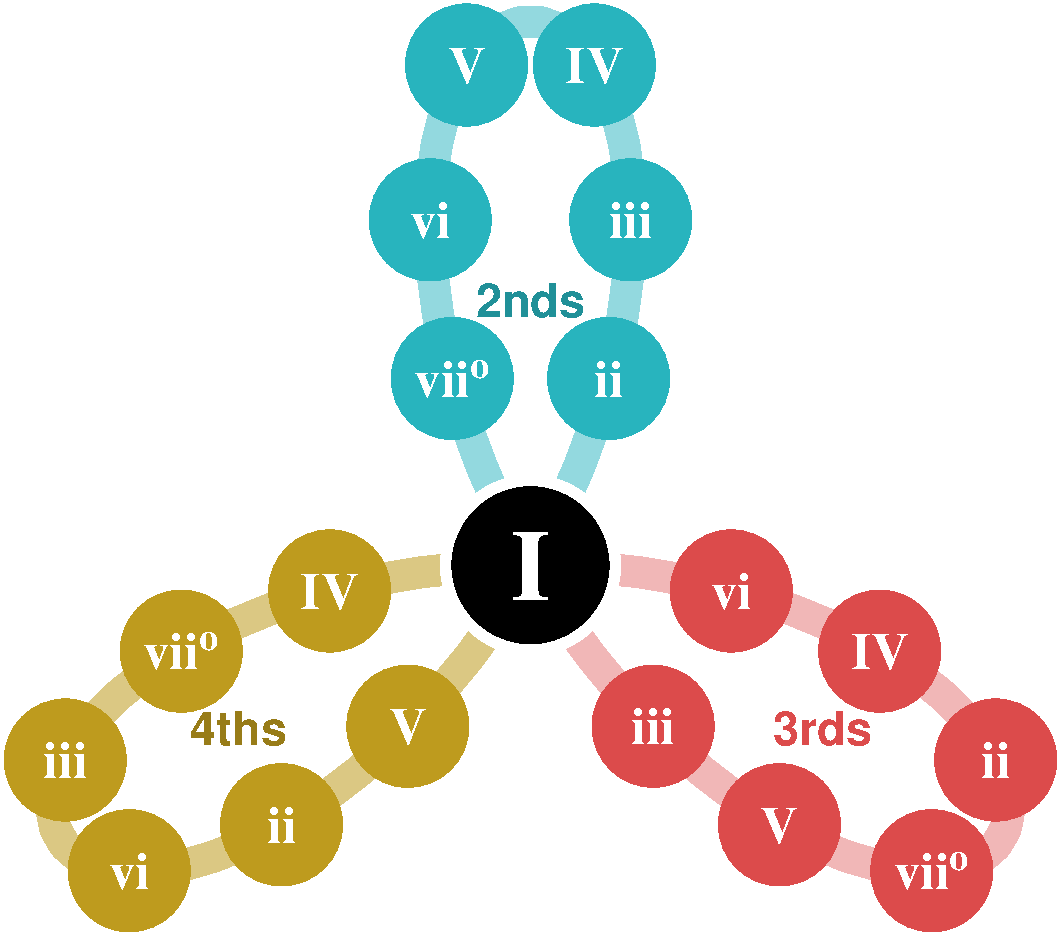
\includegraphics[width=75mm]{handout/trefoil_diag.pdf}
\par\vspace{1mm}
\setlength{\tabcolsep}{4pt}
\renewcommand{\arraystretch}{1.15}
\begin{tabular}{@{}l l l@{}}
\cyc{leafcyan!80!black}{2nd}
\tx{I}{}{ii}{}{Cloudy}{Grounding}
\tx{ii}{}{iii}{}{Deepening}{Easing}
\tx{iii}{}{IV}{}{Warming}{Cooling}
\tx{IV}{}{V}{}{Tensing}{Calming}
\tx{V}{}{vi}{}{Deceptive}{Pivoting}
\tx{vi}{}{vii}{°}{Darkening}{Reposing}
\tx{vii}{°}{I}{}{Releasing}{Fracturing}

\cyc{leafred}{3rd}
\tx{I}{}{iii}{}{Drifting}{Homecoming}
\tx{iii}{}{V}{}{Galvanizing}{Retreating}
\tx{V}{}{vii}{°}{Fraying}{Steadying}
\tx{vii}{°}{ii}{}{Tilting}{Curdling}
\tx{ii}{}{IV}{}{Gladdening}{Shading}
\tx{IV}{}{vi}{}{Grieving}{Consoling}
\tx{vi}{}{I}{}{Triumphing}{Brooding}

\cyc{leafyellow!80!black}{4th}
\tx{I}{}{IV}{}{Exploring}{Landing}
\tx{IV}{}{vii}{°}{Alarming}{Quieting}
\tx{vii}{°}{iii}{}{Despairing}{Rooting}
\tx{iii}{}{vi}{}{Accepting}{Reverting}
\tx{vi}{}{ii}{}{Wandering}{Dreaming}
\tx{ii}{}{V}{}{Lifting}{Stepping}
\tx{V}{}{I}{}{Resolving}{Lofting}
\end{tabular}
\end{minipage}

\clearpage

% ═══════════════════════════════════════════════════════════════════════════════
% PAGE 2 — Cycle preview voicings + Stacked chords
% ═══════════════════════════════════════════════════════════════════════════════

\small
\setcounter{rowct}{0}


% Header row macro for each cycle table — args: color
\newcommand{\cychdr}[1]{%
  \rowcolor{#1}%
  {\color{white}\textbf{LH}} & {\color{white}\textbf{RH}} & {\color{white}\textbf{Figure}} & {\color{white}\textbf{CW}} & {\color{white}\textbf{CCW}} & {\color{white}\textbf{Id}} \\
}

\setlength{\tabcolsep}{2pt}\renewcommand{\arraystretch}{1.15}

% Helper: rotated cycle-label cell spanning all 14 data rows
\newcommand{\cyccol}[2]{\multirow{14}{*}{\rotatebox[origin=c]{90}{\color{white}\textbf{#1}}}\hspace{0pt}}

\begin{center}
\rowcolors{2}{white}{bandcol}
\setlength{\tabcolsep}{3pt}
\begin{tabular}{@{}>{\centering\arraybackslash}m{3mm} lllll >{\centering\arraybackslash}m{3mm} lllll >{\centering\arraybackslash}m{3mm} lllll@{}}
\rowcolor{headerbg}
\cellcolor{leafcyan!80!black} & {\color{white}\textbf{LH}} & {\color{white}\textbf{RH}} & {\color{white}\textbf{Figure}} & {\color{white}\textbf{CW}} & {\color{white}\textbf{CCW}}
& \cellcolor{leafred} & {\color{white}\textbf{LH}} & {\color{white}\textbf{RH}} & {\color{white}\textbf{Figure}} & {\color{white}\textbf{CW}} & {\color{white}\textbf{CCW}}
& \cellcolor{leafyellow!80!black} & {\color{white}\textbf{LH}} & {\color{white}\textbf{RH}} & {\color{white}\textbf{Figure}} & {\color{white}\textbf{CW}} & {\color{white}\textbf{CCW}} \\
\cellcolor{leafcyan!80!black} & \sexcA{ii}{}{I}{}{Cloudy}{Grounding}{133}{933}
& \cellcolor{leafred} & \sexcB{iii\inv{1}}{}{I}{}{Drifting}{Homecoming}{133}{743}
& \cellcolor{leafyellow!80!black} & \sexcC{IV}{}{I}{}{Exploring}{Landing}{133}{B33} \\
\cellcolor{leafcyan!80!black} & \sexcA{iii}{}{ii}{}{Deepening}{Easing}{233}{A33} & \cellcolor{leafred} & \sexcB{V}{}{iii}{}{Galvanizing}{Retreating}{333}{C33} & \cellcolor{leafyellow!80!black} & \sexcC{vii}{°}{IV}{}{Alarming}{Quieting}{433}{E33} \\
\cellcolor{leafcyan!80!black} & \sexcA{IV}{}{iii}{}{Warming}{Cooling}{333}{B33} & \cellcolor{leafred} & \sexcB{vii}{°}{V}{}{Fraying}{Steadying}{533}{E33} & \cellcolor{leafyellow!80!black} & \sexcC{iii}{}{vii}{°}{Despairing}{Rooting}{733}{H33} \\
\cellcolor{leafcyan!80!black} & \sexcA{V}{}{IV}{}{Tensing}{Calming}{433}{C33} & \cellcolor{leafred} & \sexcB{ii}{}{vii}{°}{Tilting}{Curdling}{733}{G33} & \cellcolor{leafyellow!80!black} & \sexcC{vi}{}{iii}{}{Accepting}{Reverting}{333}{D33} \\
\cellcolor{leafcyan!80!black} & \sexcA{vi}{}{V}{}{Deceptive}{Pivoting}{533}{D33} & \cellcolor{leafred} & \sexcB{IV}{}{ii}{}{Gladdening}{Shading}{233}{B33} & \cellcolor{leafyellow!80!black} & \sexcC{ii}{}{vi}{}{Wandering}{Dreaming}{633}{G33} \\
\cellcolor{leafcyan!80!black} & \sexcA{vii}{°}{vi}{}{Darkening}{Reposing}{633}{E33} & \cellcolor{leafred} & \sexcB{vi}{}{IV}{}{Grieving}{Consoling}{433}{D33} & \cellcolor{leafyellow!80!black} & \sexcC{V}{}{ii}{}{Lifting}{Stepping}{233}{C33} \\
\cellcolor{leafcyan!80!black}\smash{\rotatebox{90}{\color{white}\scshape cycle 2nd}} & \sexcA{I}{}{vii}{°}{Releasing}{Fracturing}{733}{F33} & \cellcolor{leafred}\smash{\rotatebox{90}{\color{white}\scshape cycle 3rd}} & \sexcB{I}{}{vi}{}{Triumphing}{Brooding}{633}{F33} & \cellcolor{leafyellow!80!black}\smash{\rotatebox{90}{\color{white}\scshape cycle 4th}} & \sexcC{I}{}{V}{}{Resolving}{Lofting}{533}{F33} \\
\cellcolor{leafcyan!80!black} & \sexcA{ii}{7}{I}{}{Cloudy}{Grounding}{133}{9333} & \cellcolor{leafred} & \sexcB{iii}{7}{I}{6}{Drifting}{Homecoming}{1332}{A333} & \cellcolor{leafyellow!80!black} & \sexcC{IV}{Δ}{I}{}{Exploring}{Landing}{133}{B333} \\
\cellcolor{leafcyan!80!black} & \sexcA{iii}{}{ii}{s2}{Deepening}{Easing}{224}{A33} & \cellcolor{leafred} & \sexcB{V}{}{iii\inv{2}}{}{Galvanizing}{Retreating}{534}{C33} & \cellcolor{leafyellow!80!black} & \sexcC{vii}{ø7}{IV}{}{Alarming}{Quieting}{433}{E333} \\
\cellcolor{leafcyan!80!black} & \sexcA{IV}{}{iii}{s4}{Warming}{Cooling}{342}{B33} & \cellcolor{leafred} & \sexcB{vii}{°}{V}{q}{Fraying}{Steadying}{544}{E33} & \cellcolor{leafyellow!80!black} & \sexcC{iii}{}{vii}{+8}{Despairing}{Rooting}{7334}{H33} \\
\cellcolor{leafcyan!80!black} & \sexcA{V}{7}{IV\inv{2}\rp\osf{8}}{}{Tensing}{Calming}{1433}{C333} & \cellcolor{leafred} & \sexcB{ii}{}{vii}{ø7i}{Tilting}{Curdling}{6233}{G33} & \cellcolor{leafyellow!80!black} & \sexcC{vi}{}{iii}{s4}{Accepting}{Reverting}{342}{D33} \\
\cellcolor{leafcyan!80!black} & \sexcA{vi}{}{V}{+8}{Deceptive}{Pivoting}{5334}{D33} & \cellcolor{leafred} & \sexcB{IV}{}{ii}{q7}{Gladdening}{Shading}{2444}{B33} & \cellcolor{leafyellow!80!black} & \sexcC{ii}{}{vi}{7}{Wandering}{Dreaming}{6333}{G33} \\
\cellcolor{leafcyan!80!black} & \sexcA{vii}{ø7}{vi}{}{Darkening}{Reposing}{633}{E333} & \cellcolor{leafred} & \sexcB{vi}{}{IV\inv{1}}{}{Grieving}{Consoling}{143}{D33} & \cellcolor{leafyellow!80!black} & \sexcC{V}{}{ii}{7}{Lifting}{Stepping}{2333}{C33} \\
\cellcolor{leafcyan!80!black} & \sexcA{I}{+8}{vii}{°}{Releasing}{Fracturing}{733}{F334} & \cellcolor{leafred} & \sexcB{I}{}{vi}{7iii}{Triumphing}{Brooding}{5434}{F33} & \cellcolor{leafyellow!80!black} & \sexcC{I}{}{V}{6}{Resolving}{Lofting}{5332}{F33} \\
\end{tabular}
\end{center}

\vspace{2mm}

\fontsize{11}{13}\selectfont
\setlength{\tabcolsep}{3pt}\renewcommand{\arraystretch}{1.1}
\begin{center}
\rowcolors{2}{white}{bandcol}
\begin{tabular}{@{}l l l l >{\columncolor{headerbg}}m{2mm} l l l l >{\columncolor{headerbg}}m{2mm} l l l l >{\columncolor{headerbg}}m{2mm} l l l l@{}}
\rowcolor{headerbg}
{\color{white}\textbf{LH}} & {\color{white}\textbf{RH}} & {\color{white}\textbf{Figure}} & {\color{white}\textbf{Name}} & & {\color{white}\textbf{LH}} & {\color{white}\textbf{RH}} & {\color{white}\textbf{Figure}} & {\color{white}\textbf{Name}} & & {\color{white}\textbf{LH}} & {\color{white}\textbf{RH}} & {\color{white}\textbf{Figure}} & {\color{white}\textbf{Name}} & & {\color{white}\textbf{LH}} & {\color{white}\textbf{RH}} & {\color{white}\textbf{Figure}} & {\color{white}\textbf{Name}} \\
\spt{I}{}{ii}{}{133}{933}{Warm} & \cellcolor{headerbg} & \spt{ii}{}{I}{}{233}{833}{Plain} & \cellcolor{headerbg} & \spt{IV}{}{I}{Δ}{433}{8333}{Glowing} & \cellcolor{headerbg} & \spt{V}{7}{ii\inv{1}}{}{5333}{D43}{Sultry} \\
\spt{I}{}{ii}{7}{133}{9333}{Ethereal} & \cellcolor{headerbg} & \spt{ii}{}{iii}{}{233}{A33}{Mournful} & \cellcolor{headerbg} & \spt{IV}{}{IV}{s2}{433}{B24}{Hollow} & \cellcolor{headerbg} & \spt{V}{7}{ii}{7}{5333}{G333}{Smooth} \\
\spt{I}{}{iii\inv{1}}{}{133}{743}{Soft} & \cellcolor{headerbg} & \spt{ii}{}{IV\inv{1}}{}{233}{843}{Modal} & \cellcolor{headerbg} & \spt{IV}{}{V}{}{433}{C33}{Lifting} & \cellcolor{headerbg} & \spt{V}{7}{IV}{}{5333}{B33}{Pending} \\
\spt{I}{}{IV\inv{2}}{}{133}{634}{Hazy} & \cellcolor{headerbg} & \spt{ii}{}{V\inv{2}}{}{233}{734}{Floating} & \cellcolor{headerbg} & \spt{IV}{}{vi\inv{1}}{}{433}{A43}{Comforting} & \cellcolor{headerbg} & \spt{V}{7}{IV}{Δ}{5333}{B333}{Hip} \\
\spt{I}{}{V}{}{133}{533}{Bright} & \cellcolor{headerbg} & \spt{ii}{}{vi}{}{233}{633}{Rich} & \cellcolor{headerbg} & \spt{IV}{}{IV}{+8}{433}{B334}{Ringing} & \cellcolor{headerbg} & \spt{V}{7}{I}{Δ}{5333}{F333}{Leading} \\
\spt{I}{}{V}{7i}{133}{7332}{Bluesy} & \cellcolor{headerbg} & \spt{ii}{}{ii}{+8}{233}{9334}{Pealing} & \cellcolor{headerbg} & \spt{IV}{Δ}{ii\inv{2}}{}{4333}{B34}{Sparkling} & \cellcolor{headerbg} & \spt{V}{7}{V}{}{5333}{C33}{Thunderous} \\
\spt{I}{}{vi}{}{133}{633}{Pastoral} & \cellcolor{headerbg} & \spt{ii}{7}{I}{}{2333}{833}{Introspective} & \cellcolor{headerbg} & \spt{IV}{Δ}{iii}{}{4333}{A33}{Prismatic} & \cellcolor{headerbg} & \spt{V}{7}{vi}{}{5333}{D33}{Exotic} \\
\spt{I}{}{vii}{°}{133}{733}{Piercing} & \cellcolor{headerbg} & \spt{ii}{7}{IV}{}{2333}{B33}{Open jazz} & \cellcolor{headerbg} & \spt{IV}{Δ}{V}{}{4333}{C33}{Gleaming} & \cellcolor{headerbg} & \spt{vi}{}{I\inv{1}}{}{633}{C43}{Gentle} \\
\spt{I}{}{I}{s2}{133}{824}{Open} & \cellcolor{headerbg} & \spt{ii}{7}{V}{}{2333}{C33}{Hinting} & \cellcolor{headerbg} & \spt{V}{}{I\inv{2}}{}{533}{A34}{Unresolved} & \cellcolor{headerbg} & \spt{vi}{}{ii\inv{2}}{}{633}{B34}{Sprawling} \\
\spt{I}{}{I}{s4}{133}{842}{Suspended} & \cellcolor{headerbg} & \spt{iii}{}{I}{}{333}{833}{Thoughtful} & \cellcolor{headerbg} & \spt{V}{}{ii}{}{533}{933}{Punchy} & \cellcolor{headerbg} & \spt{vi}{}{iii}{}{633}{A33}{Somber} \\
\spt{I}{}{I}{Δ}{133}{8333}{Radiant} & \cellcolor{headerbg} & \spt{iii}{}{IV}{}{333}{B33}{Dark} & \cellcolor{headerbg} & \spt{V}{}{iii}{}{533}{A33}{Bouncy} & \cellcolor{headerbg} & \spt{vi}{}{IV}{}{633}{B33}{Wistful} \\
\spt{I}{}{I}{+8}{133}{8334}{Chiming} & \cellcolor{headerbg} & \spt{iii}{}{V\inv{1}}{}{333}{943}{Ancient} & \cellcolor{headerbg} & \spt{V}{}{IV}{}{533}{B33}{Coasting} & \cellcolor{headerbg} & \spt{vi}{}{V}{}{633}{C33}{Haunting} \\
\spt{I}{Δ}{I}{}{1333}{833}{Anchored} & \cellcolor{headerbg} & \spt{iii}{}{vi\inv{1}}{}{333}{834}{Pensive} & \cellcolor{headerbg} & \spt{V}{}{V}{q}{533}{C44}{Modern} & \cellcolor{headerbg} & \spt{vi}{}{vii}{°}{633}{E33}{Mysterious} \\
\spt{I}{Δ}{ii}{}{1333}{933}{Lush} & \cellcolor{headerbg} & \spt{iii}{}{vii}{°}{333}{733}{Strained} & \cellcolor{headerbg} & \spt{V}{}{V}{s2}{533}{C24}{Airborne} & \cellcolor{headerbg} & \spt{vi}{}{vi}{+8}{633}{D334}{Resonant} \\
\spt{I}{Δ}{iii}{}{1333}{A33}{Airy} & \cellcolor{headerbg} & \spt{iii}{}{iii}{+8}{333}{A334}{Tolling} & \cellcolor{headerbg} & \spt{V}{}{V}{s4}{533}{C42}{Urgent} & \cellcolor{headerbg} & \spt{vi}{7}{I}{}{6333}{F33}{Cradling} \\
\spt{I}{Δ}{IV}{}{1333}{B33}{Shimmer} & \cellcolor{headerbg} & \spt{iii}{m7}{ii}{}{3333}{933}{Layered} & \cellcolor{headerbg} & \spt{V}{}{vi}{}{533}{D33}{Velvety} & \cellcolor{headerbg} & \spt{vi}{7}{V}{}{6333}{C33}{Pointing} \\
\spt{I}{Δ}{V\inv{1}}{}{1333}{943}{Soulful} & \cellcolor{headerbg} & \spt{IV}{}{I}{}{433}{833}{Spacious} & \cellcolor{headerbg} & \spt{V}{}{vii}{°i}{533}{B43}{Sharp} & \cellcolor{headerbg} & \spt{vii}{°}{IV}{}{733}{B33}{Tangled} \\
\spt{I}{Δ}{V}{7ii}{1333}{9323}{Poised} & \cellcolor{headerbg} & \spt{IV}{}{ii}{}{433}{933}{Dreamy} & \cellcolor{headerbg} & \spt{V}{}{V}{+8}{533}{C334}{Sonorous} & \cellcolor{headerbg} & \spt{vii}{°}{vii}{+8}{733}{E334}{Twinkling} \\
\spt{I}{Δ}{vii}{°}{1333}{733}{Crystalline} & \cellcolor{headerbg} & \spt{IV}{}{iii}{}{433}{A33}{Elegant} & \cellcolor{headerbg} & \spt{V}{7}{I}{}{5333}{F33}{Commanding} & \cellcolor{headerbg} & \spt{vii}{ø7}{vi}{}{7333}{D33}{Turbulent} \\
\end{tabular}
\end{center}

\end{document}
